\graphicspath{{chapters/1_basicfeatures/figures/}}

\chapter{Basic features of the template}
\section{Compilation}
To compile the thesis, generate the bibliography, and ensure flawless cross-references between the table of contents, main text, citations, and bibliography, run
\begin{lstlisting}
lualatex -synctex=1 -interaction=nonstopmode main_thesis.tex
biber main_thesis
lualatex -synctex=1 -interaction=nonstopmode main_thesis.tex
lualatex -synctex=1 -interaction=nonstopmode main_thesis.tex
\end{lstlisting}
Of course, running these four commands manually every time is unnecessary. All \LaTeX editors I ever used (Sublime Text, VS Code, TeXstudio, TeXmaker, TeXShop, and Overleaf), allow you to set \verb|lualatex| as the default compiler and \verb|biber| as the bibliography processor. Additionally, all these editors enable you to define this sequence of commands as the standard build process to compile the document correctly with a single action.
For example, in VS Code, add 
\begin{lstlisting}
"name": "lualatex -> biber -> lualatex * 2",
  "tools": [
    "lualatex",
    "biber",
    "lualatex",
    "lualatex"
  ]
\end{lstlisting}
to \verb|"latex-workshop.latex.recipes"| in the \verb|settings.json| file.
Furthermore, the (optional) options \verb|-synctex=1 ...| are often the default choice with which the \verb|lualatex| command is run.

\paragraph{lualatex} 
This template uses \verb|lualatex| instead of \verb|pdflatex| for two reasons.
(i) Font management: The \verb|fontspec| package handles font type selection (e.g., sans-serif for captions). This requires \verb|lualatex| for compilation.
(ii) Memory management: \verb|lualatex| has a superior memory allocation system that dynamically adjusts as needed. This is important when creating figures with TikZ/pgfplots, where even simple surface plots yield out-of-memory errors with \verb|pdflatex|.

Beyond this, \verb|lualatex| offers other advantages, such as powerful Lua scripting capabilities. If you're interested, you can find numerous discussions on its benefits on \href{tex.stackexchange.com}{TeX Stack Exchange}.

\paragraph{biber and biblatex}
This template uses \verb|biblatex| with the \verb|biber| backend instead of \verb|bibtex|. \verb|biblatex| is more modern and versatile. The continued popularity of \verb|bibtex| is likely due to (bad) habit, both among users and some journals that still mandate its use.
For a thesis with a simple bibliography, \verb|bibtex| is sufficient. However, \verb|biblatex| makes customization easier. For more complex bibliography structures (e.g., the CRC183 proposal with multiple independent bibliographies, cross-references between them, chapter-specific citation highlighting, and automatic correction of incorrect entries) \verb|bibtex| is often inadequate. See \chapref{chap:biblatex} for details.

\section{Documentclass}
This template is built on the \href{https://ctan.org/pkg/koma-script?lang=de}{KOMA-script} class \verb|scrbook| \cite{koma_manual}. Whether to use the standard \verb|book| class or its KOMA-Script counterpart is largely a matter of personal preference. The KOMA-Script bundle is widely recognized as an excellent package, and personally, I find \verb|scrbook| easier to customize while also preferring its default layout.

The document class is loaded with the following options, some of which are explained below:
\begin{lstlisting}
\documentclass[numbers=noenddot, headinclude = true,
	BCOR = 12mm, DIV = 16, twoside]{scrbook}
\end{lstlisting}

\subsection{Page layout without the \texttt{geometry} package}
One of the key strengths of the KOMA-Script classes is their built-in handling of type area and other typographic settings. The package author has extensive expertise in typography and has incorporated many best practices directly into its implementation. The KOMA-Script manual states:
 ``Various algorithms and heuristic methods for constructing an appropriate type area have been discussed in the literature. These rules are known as the `canons of page construction.' [\ldots] The result is that the aspect ratio of the type area corresponds to the proportions of the page. [\ldots] In a two-sided document (e.g. a book), however, the entire inner margin (the margin at the spine) should be the same size as each of the two outer margins''\cite{koma_manual}.

The scrbook class automatically generates margins that conform to these typographic principles. The DIV parameter controls the type area width: the larger the value, the smaller the margins. The underlying construction mechanism is explained in Section 2.2 of the KOMA-Script manual, particularly in Figure 2.1.

Furthermore, \verb|headinclude=true| ensures that the header is included in the type area calculations as part of the text, and \verb|BCOR=12mm| adds a binding correction to the inner margin.

The KOMA-Script eliminates the need for the \verb|geometry| package that is otherwise often used to adjust margins. Manually setting margins can unintentionally violate typographic rules, potentially leading to poor readability. As the KOMA-Script manual warns, ``the practice of doing things oneself has long been widespread, but the results are often dubious because amateur typographers do not see what is wrong and cannot know what is important. This is how you get used to incorrect and poor typography. [...] Now, the objection could be made that typography is a matter of taste. When it comes to decoration, one could perhaps accept that argument, but since typography is primarily about information, not only can mistakes irritate, but they may even cause damage.''\cite{koma_manual, willberg2000}. (Sec.~2.8 of the manual with its polemic tone is definitely a nice read.)

\paragraph{A confession} After emphasizing the importance of adhering to typographic best practices, I must confess: this template violates them. Here is how and why:

For each combination of font size, font type (serif vs. sans-serif), and paper size, there is an optimal maximum number of characters per line to ensure readability. This determines the highest recommended \verb|DIV| value. The template uses \verb|DIV=16|, which exceeds the recommended value. As a result, LaTeX issues a \verb|Bad type area settings!| warning and suggests decreasing the \verb|DIV| value.
However, I deliberately chose smaller margins because I personally prefer this layout. My poor justification is that the recommended maximum character count per line is intended for inexperienced readers, whereas academic writing assumes a more advanced audience accustomed to dense text.



\section{Structure of the thesis}
According to the \href{https://mathnat.uni-koeln.de/sites/dekanat/official/Ordnungen/Promotionsordnung_2020.pdf}{`Promotionsordnung der math.-nat. Fakultät (2020)'} (P20), you must include
\begin{itemize}
	\item a cover / title page,
	\item an abstract (an English abstract is sufficient; a German version is not required, see P20),
	\item several chapters including an introduction, presentation of results, and discussion,
	\item the closing statement from §7 Absatz 8, P20, along with a list of your publications.
\end{itemize}
It is also common to include a thesis outline and acknowledgments. There is no universal consensus on where acknowledgments should be placed. Here, they appear between the bibliography and the closing statement. However, other placements, such as directly after the title page, are also common. If I were to write my thesis again, I would likely choose that option.

Additionally, you should list your referees. In the published version (i.e., the version published after your defense, not the initial submission), you must include the defense date and a statement confirming that the faculty accepted the thesis. This information should be printed on the title page or its back. Here, it is placed on the back of the title page.

A summary of the complete thesis structure is given in \tabref{tab:thesisstructure}.

\begin{table}
	\centering 
	\caption{\textbf{Structure of the thesis,} including details on page numbering conventions, the inclusion of individual sections in the internal Table of Contents (ToC) and the PDF reader's navigation pane (PDF-ToC), their placement on odd or even pages, and their internal numbering format.}
	\label{tab:thesistructure}
	\vspace{5ex}
	\begin{tabular}{lccccc} 
		\toprule
		 & page numbers & even/odd & in ToC & in PDF-ToC & numbered  \\ 
		\midrule 
		Titlepage front  & none & odd & \color{bqred}\XSolidBrush& \color{bqgreen} \CheckmarkBold &\color{bqred} \XSolidBrush\\
		Titlepage back & none & even & \color{bqred}\XSolidBrush& \color{bqred}\XSolidBrush& \color{bqred}\XSolidBrush\\
		Abstract & none & odd & \color{bqred}\XSolidBrush& \color{bqgreen}\CheckmarkBold & \color{bqred}\XSolidBrush\\
		Table of Contents & roman & odd & \color{bqred}\XSolidBrush& \color{bqgreen}\CheckmarkBold &\color{bqred} \XSolidBrush\\
		Outline & arabic & odd &\color{bqgreen} \CheckmarkBold &\color{bqgreen} \CheckmarkBold & \color{bqred}\XSolidBrush\\
		Part page & none & odd & \color{bqgreen}\CheckmarkBold & \color{bqgreen}\CheckmarkBold & roman letters\\
		Chapters & arabic & odd & \color{bqgreen}\CheckmarkBold &\color{bqgreen} \CheckmarkBold & numbers\\
		Appendices & arabic & odd & \color{bqgreen}\CheckmarkBold &\color{bqgreen} \CheckmarkBold & letters\\
		Bibliography & arabic & odd & \color{bqgreen}\CheckmarkBold & \color{bqgreen}\CheckmarkBold & \color{bqred}\XSolidBrush\\
		Acknowledgements & none & odd & \color{bqred}\XSolidBrush& \color{bqgreen}\CheckmarkBold & \color{bqred}\XSolidBrush\\
		Erklärung & none & odd & \color{bqred}\XSolidBrush&\color{bqgreen} \CheckmarkBold & \color{bqred}\XSolidBrush\\
		\bottomrule
	\end{tabular}
\end{table}

\subsection{Frontmatter, mainmatter and page numbering}
Books are typically divided into front matter and main matter (the back matter, which includes acknowledgments and final statement, is not relevant for the following discussion since it uses \verb|\thispagestyle{empty}|
). In the main \verb|tex| document, front and main matter are initialized via \verb|\frontmatter| and \verb|\mainmatter|. The front matter contains everything preceding the main content. It is common practice to use a different page numbering style for this section, typically Roman numerals or no numbering at all, while the main matter uses Arabic numerals.
Here, the front matter starts with the title page, but I opted not to display Roman numerals on the title page and abstract. Only the table of contents carries Roman numeral page numbers. The main matter begins with the Outline chapter. 

\subsection{Table of content}
The entire front matter should not be included in the table of contents (ToC). The same applies to the acknowledgments (which are often part of the front matter) and I also excluded the closing statement. However, all these sections should appear in the PDF table of contents (PDF-ToC), i.e., the structure that is displayed in the navigation pane of most PDF readers, see \figref{fig:pdf-toc}.

\begin{figure}
	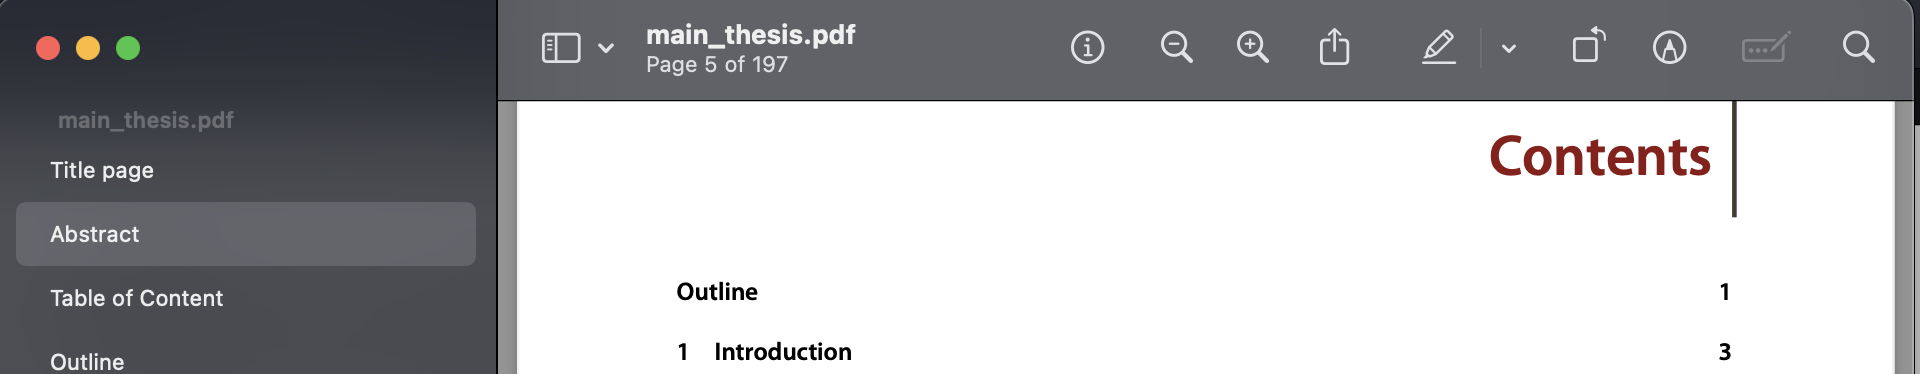
\includegraphics[width = \textwidth]{pdf-toc.png}
	\caption{\textbf{Table of content vs. pdf table of content.} Thesis parts like the title page, abstract or acknowledgments should not be typeset in the table of content. However, for ease of navigation, it is useful if they appear in the navigation panel of the pdf reader, as demonstrated here.}
	\label{fig:pdf-toc}
\end{figure}

To customize the appearance of both, ToC and PDF-ToC, the following commands are used:
\begin{itemize}
	\item \verb|\addcontentsline{toc}{chapter}{name}|  manually adds an entry to the ToC.  For example, \verb|\addcontentsline{toc}{chapter}{Bibliography}| ensures that the bibliography appears as a separate chapter in the ToC.
	\item \verb|\pdfbookmark[level]{Abstract}{abstract}| adds an entry to the PDF-ToC.
	\item \verb|\phantomsection| is sometimes necessary to fix hyperlinks between the PDF-ToC and the main document.
	\item \verb|\addchap{Outline}| ensures that the unnumbered Outline chapter appears both in the PDF-ToC and the ToC.
\end{itemize} 

\paragraph{Level of content}
Use \verb|\setcounter{tocdepth}{<depth>}| to control the number of levels displayed in the ToC.

\paragraph{Fixing the level in the PDF-ToC}
In some cases, you may need to adjust the level at which an entry appears in the PDF-ToC. For example, consider the following example thesis structure:
\begin{lstlisting}
\part{Part I}
	\chapter{Chapter 1}
\part{Part II}
	\chapter{Chapter 2}
\chapter{Conclusion}
\end{lstlisting}
The conclusion chapter is treated as a subchapter of Part II, but you may prefer it to appear on the \verb|\part| level. Here are two fixes:
Before \verb|\chapter{Conclusion}|, insert
\begin{lstlisting}
\makeatletter
\def\toclevel@chapter{-1}
\makeatother
\chapter{Concluding discussion}
\end{lstlisting}
or load the bookmark package and insert
\begin{lstlisting}
\usepackage{bookmark}
...

\bookmarksetup{startatroot}
\chapter{Conclusion}
\end{lstlisting}


\section{Folder structure of the template}
The root folder contains the main file (\verb|main_thesis.tex|), font files, \verb|.gitignore| and four subfolders: \verb|latex/| for style and setting files, \verb|auxiliary/| for front and back matter content, \verb|bib-files/| for \verb|.bib| files and \verb|chapters/| for the main content.
See \figref{fig:folderstructure} for a concise overview, including the substructure of \verb|chapters/|.

\begin{figure}
\begin{forest}
	for tree = {inner sep=0pt,l=40pt},
  pic dir tree,
  where level=0{}{% folder icons by default; override using file for file icons
    directory,
  },
  [root
    [main\_thesis.tex, file]
    [\fname{auxiliary}{files for front and back matter}
      [\fname{abstract.tex}{one file for each part of the front/back matter: title page, abstract, \ldots.}, file]
      [\fname{logos}{Logos for title page, not included due to license issues.}]
    ]
    [\fname{bib-files}{files with \texttt{bibtex}/\texttt{biblatex} entries}
    	[\fname{bibliography1.bib}{.bib files}, file]
    ]
    [\fname{chapters}{main content}
    	[1\_introduction
    		[\fname{1\_introduction.tex}{main tex file for chapter 1}, file]
    		[\fname{figures}{figures for chapter 1}]
    		[\fname{tikz\_figures}{TikZ source code for figures in chapter 1}
    		[\fname{tikz\_chap1\_fig1.tex}{A \texttt{tex} file for each figure in chapter 1}, file]
    		[\fname{data}{Data used by \texttt{tikz\_chap1\_fig1.tex}}]
    		]
    	]
    	[\fname{...}{one folder for each chapter with equal substructure}]
    	[outline.tex, file]
    ]
    [\fname{latex}{layout/style definitions}
    	[\fname{layout.tex}{layout settings}, file]
    	[\fname{...}{more files for TikZ styles, color definitions, custom \LaTeX commands, \texttt{biblatex} settings, etc.}, file]
    ]
    [.gitignore, file]
    [\fname{otf/ttf files}{font files, not included in template}, file]
  ]
\end{forest}
\caption{\textbf{Structure of the root folder of the template.} The root folder contains the main file, font files, Git files, and four subfolders, two of which hold the actual content: \texttt{auxiliary} (for front and back matter) and \texttt{chapters} (for the main matter). The \texttt{chapters} folder includes a separate subfolder for each individual chapter, including the appendices. Each of these subfolders follows the same structure, containing a main \texttt{tex} file for the chapter, a \texttt{figures} folder, and, if TikZ/pgfplots is used, an optional \texttt{tikz\_figures} folder for the TikZ source code (with one file per figure) and associated data.}
\label{fig:folderstructure}
\end{figure}

After \verb|\begin{document}|, all \verb|tex| files are imported using \verb|\include{filename}|. To compile only specific parts of the thesis, add \verb|\includeonly{filename1,filename2,...}| to the preamble. \verb|\include| generates separate \verb|.aux| files, ensuring that pages, chapter, and other numbering remain correct. However, this is usually not a major concern during the writing process and using \verb|\import{filename}| instead is also perfectly fine.

At the beginning of each chapter, it is useful to set the graphics path to the corresponding figure folder (e.g., \verb|\graphicspath{{chapters/1_basicfeatures/figures/}}| for this chapter) such that the full path can be ommited when using \verb|\includegraphics|.

\section{Using TikZ / pgfplots and externalization}
When using TikZ/pgfplots, it's highly recommended to enable TikZ's externalization feature to avoid re-rendering of unchanged figures with every compilation. This saves a significant(!) amount of time.  
Make sure to include \verb|\usepackage{shellesc}| and compile with the \verb|--shell-escape| flag. In addition, there are two template-specific pecularities to keep in mind: 

\paragraph{Chapter headings} The modified chapter heading relies on TikZ, so TikZ externalization should be disabled at the beginning of each new chapter. To automate this, simply uncomment the following code snippet in the preamble of \verb|main_thesis.tex|:
\begin{lstlisting}
\let\oldchapter\chapter	% Store \chapter in \oldchapter
\renewcommand{\chapter}{%
	\tikzexternaldisable
	\oldchapter%
}
\end{lstlisting}
\paragraph{Folder structure}
Additional \verb|tikz_figures| folders store a separate \verb|tex| file with the TikZ source code for every figure. This folder contains a \verb|data/| subfolder with the data required by the source files. To simplify figure inclusion, I set up paths at the beginning of each chapter, e.g.,
\begin{lstlisting}
\renewcommand{\here}{chapters/3_colors/tikz_figures} %Path to TiKz source code
\pgfplotsset{table/search path={\here/data}} %Path to data used in TikZ source code
\tikzsetexternalprefix{chapters/3_colors/figures/} %Path for externalized tikz pdfs.
\end{lstlisting}
The \verb|\here| command is originally defined in the document preamble
Then, to include a TikZ figure use
\begin{lstlisting}
\begin{figure}
	\centering
	\tikzsetnextfilename{fig_colordemo}
	\input{\here/tikz_colordemo.tex}
	\caption{Some caption} \label{fig:colordemo}
\end{figure}
\end{lstlisting}
For an example in action, see \chapref{cha:colors}.
Of course, there are many ways to organize the folder structure, especially regarding TikZ externalization---just choose what works best for you.

\section[Layouting ``outer'' design elements]{Layouting outer design elements}

If this template has a distinctive look, it's probably due to the layout of its outer design elements, i.e., chapter and section headings, header line, and part page. If you do not want to replicate the layout entirely, the easiest approach is to customize these design elements. (But I am totally fine if you use the template as it is, see all the \href{https://www.thp.uni-koeln.de/trebst/thesisprojects.shtml}{theses published in our group after mine}, as of January 25.)
All the design elements we discuss in this section are defined in the file \verb|latex/layout.tex|. 


\subsection{Accent colors}
I use two accent colors for highlighting, cardinal red for captions and warm grey for the header and parts of the chapter headings. They can be changed in \verb|latex/layout.tex|. The default is
\begin{lstlisting}
\colorlet{accentcolor1}{warmgrey}
\colorlet{accentcolor2}{cardinalred}
\end{lstlisting}
\verb|warmgrey| and \verb|cardinalred| are defined in \verb|latex/colors.tex|. 

\subsection{Fonts}
By default, \verb|scrbook| uses a sans-serif font for captions. While I like this approach, I was not satisfied with the defaul font and used the \verb|\fontspec| package to pick Myriad Pro, the OpenType version of the \href{https://en.wikipedia.org/wiki/Myriad_(typeface)}{Myriad font family}.
Personally, I prefer the slimmer and more elegant semi-bold and regular weights over the traditional bold fonts, even for headlines. I stored the two \verb|otf| files (called \verb|myriadpro-semibold.otf| and \verb|myriadpro-regular.otf|) in the root folder. New fonts can then, e.g., be set as follows:
\begin{lstlisting}
\newfontfamily{\mainsemibold}{myriadpro-semibold.otf}
\addtokomafont{section}{\mainsemibold\Large\color{accentcolor2}}
\end{lstlisting}
Further details can be found in latex/layout.tex. This template does not contain any \verb|otf| files. Just google for them (or for the \verb|otf| or \verb|ttf| files of your favorite font).
To compile this thesis without the \verb|otf| files at hand, simply comment lines 16--18 in \verb|layout.tex| and uncomment lines 20--21. In that case, you can even omit the \verb|fontspec| package.


\subsection{Chapter headings}
The most striking feature in this template are probably the chapter headings.
The appearance of the chapter heading is defined after \verb|% Beginning of chapter style|. You can uncomment everything but the first line in the style definition to obtain the standard \verb|scrbook| chapter headings with modified font and color. People have come up with many great chapter heading styles, mine is also a modified version of one from tex.stackexchange. If you’re looking for inspiration, google for `Customizing Chapter Style in scrbook' or similar.

\paragraph{Adding linebreaks}
I wasn't always satisfied with how line breaks were handled for long chapter headings. However, manually inserting line breaks can make the title appear awkward in the table of contents (ToC). The solution is the following syntax:
\begin{lstlisting}
\chapter[Many-body localization and quantum chaos in transmon quantum computers] {Many-body localization \\ and quantum chaos \\ in transmon quantum computers}
\end{lstlisting}
The text inside the square brackets appears in the ToC, while the curly brackets define how it is displayed in the chapter itself.

\subsection{Part pages}
I don't use part pages. I considered grouping the introductory chapters into one part and the results chapters into another, but I felt this created unnatural breaks. I think part pages make sense only when dealing with disjoint topics The only real argument in favor of part pages was that they look kind of cool, but that alone wasn't convincing enough.

If you want to use part pages, here’s how: You can customize the layout by modifying the definitions after \verb|% Beginning of part page style|. One can, e.g., add a monochrome background, color gradients or a background image, see the comments in \verb|latex/layout.tex|. See part~\ref{part:examplepartpage} for an example of a part page with a (weird) color crossover.

\subsection{Sections, subsections, subsubsection and paragraphs}
The appearence of these lowerlevel headings is modified using the \verb|\addtokomafont| command. In my thesis, I never use \verb|subsubsections|, but occasionally, I use paragraphs.

\subsection{Figure captions}
The appearance of the figure captions is controlled with the \verb|caption| package that allows wide-ranging customization. For example, I wanted the font of the figure caption to be slightly smaller than the main text font. Again, see \verb|latex/layout.tex| for details and more options.

\subsection{Header}
For the header, I use the \verb|scrlayer-scrpage| package from the KOMA-script bundle. I was already very satisfied with the standard appearance (chapter on even pages, section on odd pages) and only adapted the color and the font, see \verb|latex/layout.tex|.

\subsection{Balancing figures and text}
If larges take up more than half a page, \LaTeX~may prevent any additional text from appearing on that page. I wasn't always satisfied with how \LaTeX~handled this, so I adjusted the default value of \verb|\textfraction|, which controls the minimum amount of text required on a page. I had to tweak three additional values (\verb|\floatpagefraction|, \verb|\topfraction|, \verb|\bottomfraction|) to adjust the figure placement and the balance between text and figures or tables to my wishes.
